\section{日本が狙うサイエンス}\label{galaxy.s3}

系外銀河の観測や銀河進化の研究に於ける日本の強みは、
観測的には、これまで野辺山等の観測で培って来た
電波観測の知識と経験の蓄積である。特に、
ALMAの観測時間へのアクセスがあることが実際的に
有利である。
ALMAはダストと多彩な分子を観測するのに適しており、
SKAの水素原子の観測と組み合わせることによって、
原子ガスから、分子ガスを介して、星形成と重元素汚染が
起きる、いわゆる星間ガスのリサイクルの全貌を捉える事が
できるのである。理論的にも、日本は銀河形成のシミュレーションと
銀河の化学進化モデルが強く、理論的予言は言うまでもなく、
SKAやALMAによってより暗い銀河、
より遠い銀河が見えて来た時に、その理論的解釈をいち早く提供できる
利点がある。

銀河形成研究においては、主として3つの赤方偏移の範囲が重要である。
まずは宇宙初期、ガスから星が形成されることによって銀河が成長していく、
いわば銀河の成長期($z > 3$)である。
特に星形成の前夜ともいえる、大量のガスを持った進化初期の銀河の
直接観測は銀河形成の物理の検証として本質的に重要である。
そして、階層的構造形成により銀河が銀河としてのグローバルな性質を持つように
なってゆき、ハッブル分類のような銀河の形態が出現する時代($1 < z < 2$)が
銀河進化の文脈で極めて興味深い。
この時代は銀河の合体率(merging rate)、平均的な星形成率や
ダストで隠された星軽視の割合がピークを迎える(\S~\ref{galaxy.s0.5}参照)
銀河進化の激動の時期であり、様々な物理過程が複雑に絡み合って
統一的な見解が得られるには遠く至っていない。

そして、銀河進化研究において最近とみに見落とされがちなのが$z=0$、すなわち
近傍宇宙である。
銀河進化全てに関わる過程は、「ゼロ点」である近傍宇宙の素過程と比較されて初めて
「進化」を追ったと言える。
これは全く自明なことであるが、どういうわけか最近の銀河進化研究においては研究の主流から
外れた分野と見なされる傾向があった。
また、近傍宇宙の銀河の物理の詳細を突き詰めることで星間物理とのクロスオーバーを
構築することができ、星間物理--近傍銀河--遠方銀河という道筋を一つの大きな
流れとして扱うことができるようになる。
気取った言い方をすれば、星間物理から銀河進化研究の``シルクロード''を繋いでゆく研究が
近傍銀河の物理である。
ここでは上記の日本の強みに鑑み、いくつかのサイエンス
ケースに対してどのような貢献ができるのかを、3つの代表的時期に関連して
紹介する。

\subsection{近傍銀河: 星間物質の性質$\cdot$進化、星形成の統一的理解}

ここではまず、$\sim 10\;\mbox{Mpc}$程度の距離にある近傍銀河の詳細なSKA観測にもとづく日本が
狙うべきサイエンスについて述べる。
特に、1) 最近明らかになってきた原子ガスと分子ガスの遷移層にあるdark gasの正体の解明、2)
低金属量環境下における原子ガスからの星形成、の2点について以下で述べる。
ここでの議論はSKA-JP星間物理サブグループとのシナジー研究となっている。

これまで、21~cm輝線は光学的に薄いという仮定のもと原子ガスの質量が見積もられてきた。
しかし\citet{2015ApJ...798....6F}は、Planckによる天の川銀河の詳細なダスト分布と{\sc H\,i}データの比較から、
21~cm輝線放射の50\%程度は冷たく、光学的に厚い水素原子からのものであることを示した。
この研究において、光学的に厚い水素原子こそが、21~cm輝線やCO輝線で感度のない
密度範囲$100\mbox{--}1000 \; \mbox{cm}^{-3}$のガス(dark gas)の正体である可能性を示唆している。
今後はdark gasを含む、銀河ISM進化の統一的理解のために、電離ガス・原子ガス・分子ガスの量・分布・運動状態などを銀河内・異なる銀河間で網羅的に比較することが重要である。
天の川銀河は最も詳細に調べることのできる銀河であるが、我々がその中に存在しているために、銀河の構造とISMの性質の比較をすることは容易ではない。
円盤銀河における渦状腕や棒状構造などの銀河スケールの大規模な構造は、銀河ISMの物理状態に大きな影響を与える。
今後、SKAで達成される角度分解能($\sim 0.1\; \mbox{arcsec}$)によって、2本の卓越した渦状腕を
持つ(grand-design)渦巻銀河が存在する典型的な距離10~Mpcでも5~pcの空間分解能を達成することができる。
ALMAで取得可能な近傍銀河における詳細なダスト・分子ガス分布と、SKAで取得される詳細な原子ガス分布との比較は日本が狙うべき重要なテーマの一つである。


上で述べた力学的な擾乱だけでなく、ダスト量に比例していると考えられる金属量の違いも、銀河ISMの物理状態に
影響を与える。
近年の星形成に関する理論研究において、ISMが分子ガスの状態であることは星形成の必要十分条件ではなく、低金属量な環境下では原子ガスからも星形成をする可能性が示唆されている。
矮小銀河や円盤銀河外縁部などの近傍の低金属量環境下での原子ガスの性質の詳細な理解もまた、SKAで行うべきサイエンスの一つである。
以下では、この分野についてわかりやすく、簡潔にレビューしている\citet{krumholtz2013}をもとに、
水素原子--水素分子間の遷移と星形成に関して紹介する。

原子ガスは分子ガスの原材料と考えられているが、近傍銀河における星形成率は、分子ガスとの相関はいいものの、原子ガスとの相関はそこまでよくない
\citep{2002ApJ...569..157W, kennicutt2007, 2008AJ....136.2846B, 2008AJ....136.2782L}。
なお、分子ガス質量を星形成率で割ったdepletion time scale $t_{\rm dep}$は、近傍円盤銀河ではほぼ一定であり、2~Gyr程度であることも観測的に示されている\citep{bigiel2011}

星間水素の化学状態(原子ガスないし分子ガス)を決めているのは、Lyman-WernerバンドのUV光による
水素分子の解離と、(金属量が太陽の十万分の1程度以上ならばダスト上での水素分子形成のバランスである
\citep{omukai2010}。
太陽近傍の典型的なUVの輻射強度における水素分子の乖離率は、水素分子一つあたり$5\times 
10^{-11}\, \mbox{s}^{-1}$ \citep{1996ApJ...468..269D}であるのに対し、太陽金属量(ダスト量が金属量に
比例すると仮定\footnote{これは化学進化がある程度以上進んだ銀河ではよい近似であり、近傍銀河では
問題なく使える。低金属量銀河の場合についてはこの仮定は破れる。詳細は星間物理の章を参照。})、
水素原子の柱密度$100
\; \mbox{cm}^{-3}$における水素分子の形成率は、水素原子一つあたり$3 \times 10^{-15}\; \mbox{s}^{-1}$である。
そのため、分子解離率と分子の形成率のバランスから予想される太陽近傍における水素分子の割合は非常に
低く$10^{-4}$となってしまう。
しかし、ダストの豊富な領域ではLyman--WernerバンドのUV光子が十分に遮蔽され、水素分子の割合が1になり、分子雲が形成されると考えられる。
そのため、分子雲の典型的な構造としては、UV光の減光があまり効かない水素原子が優勢な外層、UV光の減光が効き始め水素分子が優勢な内側、という状態が期待される
\citep[e.g.,][]{van_dishoeck1986, sternberg1988, neufeld1996, liszt2002, glover2007, 2008ApJ...689..865K, 2009ApJ...697...55G, 2010ApJ...709..308M, mac_low2012}。

分子ガス--星形成率間のよい相関の理由としては、星間水素ガスの化学状態と熱状態(温度)を決めているのが、両方ともダストによる遮蔽である点が挙げられる。
まず、化学状態に関しては、(ダストによる吸収を受けつつの)Lyman--WernerバンドのUV光子による水素分子の光乖離、ダスト粒子上での水素分子形成のバランス、熱状態に関しては、やはりLyman--WernerバンドUV光子によるダストの光電効果加熱とダスト--ガス間の熱交換、衝突励起されたガスの輝線放射による冷却のバランスで決まっている。
そのため、星間水素の化学的プロセスと熱的プロセスの、ガスの体積密度、柱密度、UV輻射場強度への依存性は極めて似ている。
輝線放射による冷却と水素分子形成は両方とも、衝突によるものであり、冷却率と形成率は両者とも、密度と金属量に$n^2 Z’$という依存性を持つ。
光解離と光電効果加熱は両者とも、UV輻射場強度とダスト減光とに同じ形で依存している。

この類似性により、ガスの温度や化学状態は、幅広いガス密度、ダスト減光、金属量範囲で相関がよい。
原子ガスから分子ガスへの遷移はだいたい$>100\; \mbox{K}$から$\mbox 10\;  \mbox{K}$のところでおきるが、
これを決めているのはダストによる遮蔽である:
星間水素の大半が水素分子であるような遮蔽の効いている領域では、低温になっており、逆に遮蔽の効いていない場所では、加熱率が高いために高温となっている。
そのため、水素分子と星形成の間にはよい相関がある:
水素原子から水素分子への変換が星形成を引き起こしているわけではないが、ガス温度の低下は水素原子と水素分子間の遷移が付随するのである。

低金属量環境下では、完全な水素原子から完全に水素分子になるためのタイムスケールは力学的時間と同程度であり、熱的平衡状態になるのに必要なタイムスケールは1/1000程度と短い。
化学的タイムスケールと熱的タイムスケールは両者とも金属量に依存し、低金属量環境化では長くなる。
一方、星形成雲の力学的時間(星形成のタイムスケール)は金属量に依存しない。
そのため、$熱的タイムスケール < 力学的タイムスケール < 化学的タイムスケール$となる金属量があるはずである。
このことは、星形成を支配しているのが化学状態でなく熱状態であるとすれば、星間水素が水素分子になる前に星形成が起こるということを示している。
そのような状況下では、星形成率は水素分子ではなく水素原子と相関がよくなるはずである。
\citet{glover2012}は数値シミュレーションを行い、水素原子からの星形成の可能性を示し、\citet{krumholtz2012}は
解析的モデルをたて、太陽の金属量の1--10~\%でこの効果が見られる可能性を示した。

SKA-JP銀河進化サブグループは、ALMAとの実践的リンクという強みを生かし、近傍の様々な
金属量、進化段階の銀河について、空間的に分解した原子--分子転移を追求し、遠方銀河と
比較されるべき基準となる物理過程を明らかにすることを目指す。

\subsection{ガス、ダスト及び星形成を結ぶ拡張スケーリング則の探索と理論化}

銀河の本体が十分に形成されると、銀河の持つ諸量の間に密接な関係が出現する。
これがスケーリング則と呼ばれているもので、銀河進化研究の重要なツールとなっている。
スケーリング則のもっともよく知られている例が、\S\ref{sec:TF}において述べたTF関係、
BTF関係である。
そして銀河にはこれ以外にも様々なスケーリング則が知られている。
ところが、そのほとんどはスケーリングが成立する物理的理由が知られていない
経験的関係式である。
ここでは銀河進化と関連の深いスケーリング則を紹介し、その有機的統合と理論化への大まかな道筋について
述べる。

銀河進化の観点からは星形成率が最も興味ある物理量であり、星形成率の関係する
スケーリング則を検証したい。
2015年現在、銀河の星形成に関係するスケーリング則で最も注目されているのが
星形成銀河主系列と呼ばれる関係である。
これは銀河の星形成率(SFR)と星質量($M_*$)の間に成立する線型関係である。
歴史的に色--等級関係(color--magnitude relation)として知られている経験則と
等価であるが、銀河のカラーではなくSFRおよび$M_*$というより物理的な量を用いた
ことで、星形成率の従うスケーリングが鮮明に浮かび上がってきたのである\citep[e.g.,][]{schiminovich2007}。
どちらも銀河全体について積分量であるので、その間に自明なスケーリング則が存在
することは驚くに値しない。
注目すべきはその傾きが1よりも小さい、つまり大きな銀河ほど単位星質量当たりのSFRが
小さくなっていることである。
このことはSFRの代わりに比星形成率$\mbox{SSFR} = \mbox{SFR} / M_*$を
用いるとより鮮明に見えてくる(図~\ref{fig:sf_ms})
この傾向はダウンサイジングと呼ばれており、1980年代後半から認識されていたものの、その
物理的な意味は現在に至るまで明らかになっていない。

\begin{figure}[thbp]
\begin{center}
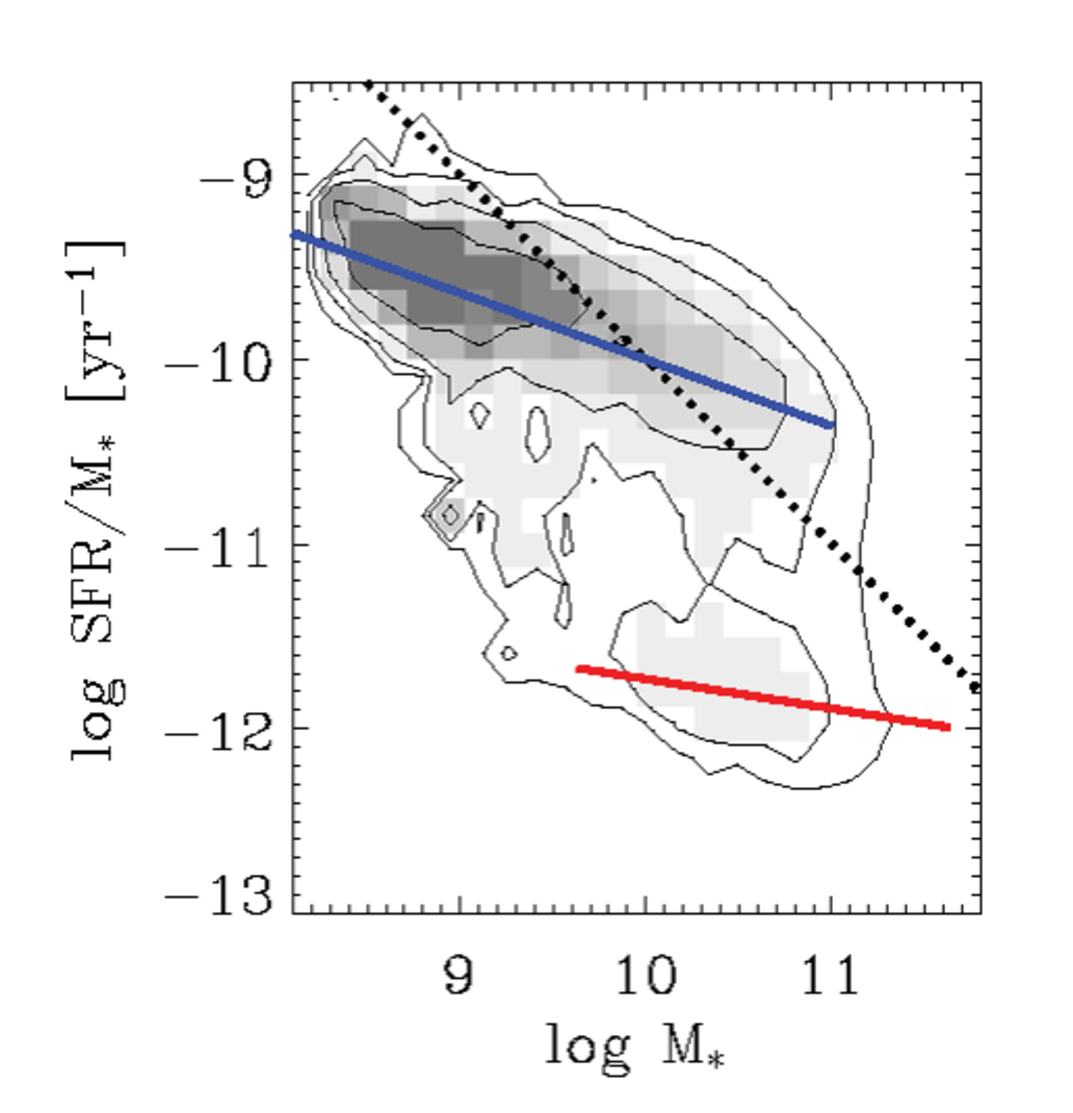
\includegraphics[width=0.5\linewidth]{galaxy/schiminovich2007.eps}
\end{center}
\vspace{-0.3cm}
\caption{{\sl GALEX}による紫外線観測で得られた星形成銀河主系列。上の線が
星形成主系列で、下の線は赤い、星形成を停止しつつある銀河(red sequence)に対応する
\citep[][より改変]{schiminovich2007}。}
\label{fig:sf_ms}
\end{figure}


高光度赤外銀河など爆発的な星形成をしている銀河は星形成銀河主系列に乗らず、
1桁以上主系列から上に分布することが知られている\citep[e.g.,][]{buat2005, buat2007}。
これは、星形成主系列が永年的進化をする銀河の道筋であるか、あるいは単に滞在時間の
長い系列であるということを意味している。
また、楕円銀河など星形成をほぼ停止した銀河は主系列から下方に外れ、$\mbox{SFR} = 0$に
至ると図上に乗らなくなる。
このことから、星形成銀河主系列を進化のトラックとして捉えるためには、様々な
側面からの研究が必要であることが分かる。
\citet{genzel2012}は星形成主系列の銀河の分子ガス量の検証を試みた。
銀河サンプルの赤方偏移は$0 < z < 2$であるが、まだケーススタディを集めている状態で、
系統的探査のレベルには至っていない。
\citet{magnelli2012}および\citet{magnelli2014}は星形成銀河主系列における
ダスト温度と分子ガス温度の関連性を研究している。
また\citet{magnelli2015}は、広く知られている銀河の赤外線--電波強度相関と
星形成主系列との関連に注目している。
しかし、中性ガスの観測が$z < 0.5$程度に限られる現在、銀河進化を視野に置いた
研究は難しい。
そして、次に述べる星形成のもう一つの重要なスケーリング則であるKennicutt--Schmidt則と
星形成銀河主系列との関係を明らかにするためには、銀河を空間分解して観測することが
不可欠となる\citep{teruya2014}。
このように、星形成銀河主系列が出現する理由を星間物理的に解明する研究はALMAを経て
SKAに至る観測によって初めて可能になる。

\begin{figure}[htb]
\begin{center}
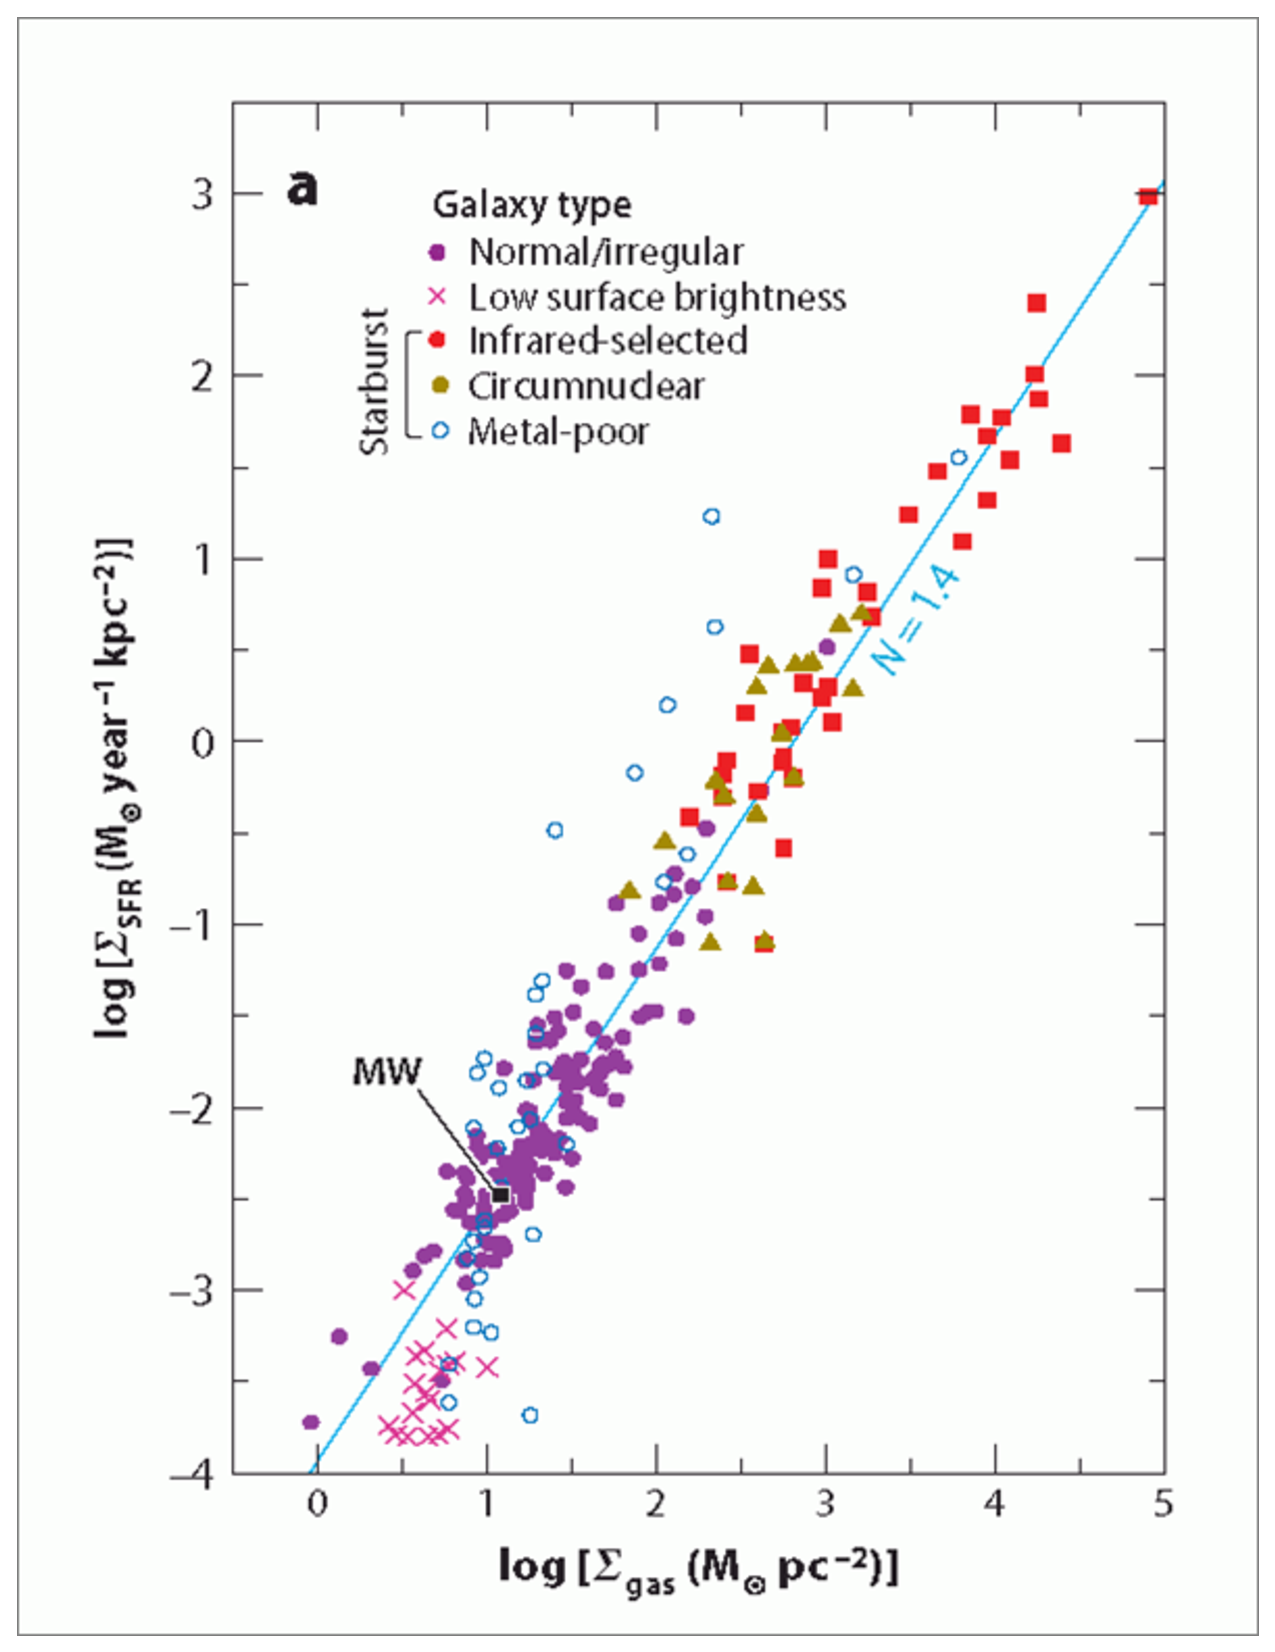
\includegraphics[width=0.5\linewidth]{galaxy/KS_relation.eps}
\end{center}
\caption{Kennicutt--Schmidt則。ガス面密度$\Sigma_{\rm gas}$、SFR面密度$\Sigma_{\rm SFR}$とも
7桁近い範囲で成立する単一冪型の関係である\citep[][]{kennicutt2012}。}
\label{fig:ks}
\end{figure}

銀河における星形成の物理は比較的局所的な物理条件が関係する現象である。
ところが、古くから銀河の大域的性質と星形成が関係することが知られている\citep[e.g.,][]{roberts1994,kennicutt2012}。
銀河の渦状腕や分子雲、電離水素領域といった局所的な現象と、銀河の形態や全質量などの
大域的な性質が見事に関連している理由はまったく自明のものではなく、天体物理学によって
解明されるべき重要な課題である。
局所的から大域的な様々なスケールで現れる銀河のガス(面)密度と星形成率の関係が
Kennicutt--Schmidt(KS)則である\citep[レビューとしてはたとえば][]{kennicutt2012}。
定量的にはKS則は以下のように表現される。
\begin{equation}\label{eq:ks}
  \Sigma_{\rm SFR} \propto \Sigma_{\rm gas}^n \;. 
\end{equation}
これは、ガス面密度$\Sigma_{\rm gas}$、SFR面密度$\Sigma_{\rm SFR}$ともに7桁近い
範囲で成立する単一冪型の関係である(図~\ref{fig:ks})。
ここで、係数$n$は観測的に$1 < n < 2$の範囲に入ることが知られている。
この係数が1に近いか2に近いかによって、星形成のもととなる分子ガスの物理過程について
異なったシナリオを与える\citep[e.g.,][]{momose2013}。
また、KS則は銀河の化学進化理論においては星形成史を決定する重要な構成要素であり、
銀河進化理論へのインパクトも大きい。
このように、KS則は星間物理から銀河物理にわたる多くの研究者の
興味の対象となっている。

しかし、根本的な問題として、KS則も観測から得られた純粋な経験則であることを指摘
しておかねばならない。
しかも、観測から決まる冪指数$n$についても現在議論が収束していない。
分子雲の重力崩壊や分子雲衝突などの星間過程から理論的にKS関係を求めるには、
まず十分な数の銀河サンプルから目指すべき経験則を
なるべく小さな誤差で示す必要がある。
このために、分子ガス、中性水素ガスともに十分な数があり、共通の選択基準に基づく
銀河サンプルが不可欠となる。
SKAはここにおいて他の追随を許さない重要な役割を果たす。
SKAによって得られたH\,{\sc i}セレクトの銀河サンプルを用い、空間分解されたKS則を$z \sim 1$まで
検証し、KS則を生む本質的な物理過程が何かを明らかにする。
そして、BTF関係や星形成銀河主系列と統一的に扱うことで、銀河が従う究極のスケーリング則を
見出すことができる。 
さらに、SKA-JP星間物理サブグループとのシナジーにより、この結果を星間物理から第一原理的に導く
ことを試みる。
ここまで来て初めて、銀河進化研究も天体物理学として成熟することになるだろう。



\subsection{水素原子21 cm吸収線系で探る銀河進化}\label{galaxy.s3.ss1}

\ref{sec:DLA}節と\ref{subsec:international_21cm}節で述べた様に、
クエーサー等の明るい連続光源を利用して、その視線上にあるガスを
吸収線で検出する事により、そのガスが附随する銀河および銀河間ガスの構造
の宇宙論的時間スケールでの進化を研究する事ができる。特に、地上の
可視望遠鏡でサンプルできる
水素Ly$\alpha$吸収線系はこれまでにも盛んに研究されてきた。最近は
電波望遠鏡を用い、水素の21 cm吸収を、既にLy$\alpha$で
サンプルされた吸収線系、特に柱密度の大きな%damped Ly$\alpha$雲
DLAをターゲットにして観測する研究も行われている。
電波の連続光源自体を無バイアスにサーベイして、可視サンプルに
依らない電波独自の吸収線サンプルを得る事も国際的にSKAでの
主要な科学目標として提案されている。

吸収線系の物理状態を観測的に明らかにするためには、Ly$\alpha$以外の
吸収線も同定することが重要である。例えば、重元素の吸収線から
求められる重元素の組成比は、銀河進化の
重要な側面である化学進化を特徴づける重要な量である。この
化学進化からの観点からは、日本でも、第一世代星による重元素
合成の痕跡を探る研究\citep{2011ApJ...730L..14K}や世界であまり
注目されていないNa等の重元素に着目して研究した
例\citep{2006ApJ...643..667K}等がある。銀河の化学進化は
日本でも強い分野であり、様々な
元素を横断的に用いて、理論の助けを借りながら、
吸収線系を研究していく事が今後も
期待される。

銀河スケールでの星間ガスのシミュレーションも、日本で
強い分野である。特に、吸収線系と関連する
我々独自の研究として、星間ガスの構造がどれくらい吸収線系の統計に
現れるかを理論的に研究したものがある。
%我々
\citet{2003MNRAS.341L..18H}は、$z\sim 3$で典型的に見られる
星間ガスの構造を見るために、銀河円盤の
シミュレーション\citep{2001ApJ...547..172W}に基づいた
星間ガスの構造を計算した。更に、観測との比較のために、
星間ガスの密度に敏感な
水素分子の存在比(水素分子の水素全体に占める割合)の統計を
シミュレーションされた
星間ガスの構造のもとで調べた。その結果、水素分子は、塊状の構造に
局在化されるので、水素分子の存在比の高い($\gtrsim 10^{-3}$)領域が
ちょうどクエーサーの視線上にくる確率は低い(典型的に10\%程度)。
これは、大部分のDLAで水素分子存在比が$10^{-6}$より小さく、
水素分子存在比が高い($\gtrsim 10^{-3}$) DLAがサンプル数は少ないが
大雑把に10\%程度である観測事実\citep{2003MNRAS.346..209L}を良く説明する。

\ref{sec:DLA}節で述べたように、最近DLAをサンプルとした21 cm線吸収の観測も行われて
いるが、21 cm吸収線はあまり検出されて
いない\citep{2012MNRAS.421..651S,2014MNRAS.438.2131K}。
式(\ref{eq:tau21cm})でも見たように、21 cm線の光学的厚さはガスの
スピン温度に依る。つまり、DLAで観測される小さな光学的厚さは、
温度が高い($\gtrsim 10^3$ K)ガス(warm ISM)を見ているためであると解釈される。
つまり、DLAのホスト天体は、warmガスの占める割合が大きく
coldガスの占める割合が小さいと、21 cm吸収線があまり検出されない観測事実を
うまく説明できる。Cold gasは水素分子存在比も
大きい為、cold gasの占める割合の小さな事は、水素分子の存在比の小さな
DLAが圧倒的多数を占めるという上記の観測結果と整合的である。

%我々
\citet{tee15}は、21 cm光学的厚さの分布を上記の
シミュレーション\citep{2003MNRAS.341L..18H}を基に計算した。
その結果を図\ref{fig:distri_21cm}に示す。
シミュレーションの格子点の統計を取る際に、DLAの
選択基準と同一になるよう、水素の柱密度が$2\times 10^{21}$ cm$^{-2}$
よりも大きくなる所だけを数えた。また、ダスト減光は
重元素率に比例すると仮定し、Znの柱密度が$10^{13.2}$ cm$^{-2}$
より大きな柱密度を持つ格子点は、背景にクエーサーが
あったとしても減光のためにサンプルされない\citep{2005A&A...444..461V}ので、統計から
除外した。また、線幅は典型的なdiffuse星間ガスの速度分散の
値$\Delta v=10$ km s$^{-1}$を仮定した\citep{2009ApJ...695..937B}。

\begin{figure}[thbp]
\begin{center}
\includegraphics[width=0.7\linewidth]{galaxy/Inttau_v3.eps}
\end{center}
\vspace{-0.5cm}
\caption{我々の流体シミュレーションによって予言される、
DLAホスト天体の星間ガスに典型的な21 cm光学的
厚さ($\tau_\mathrm{21~cm}$)の分布関数。実線、点線、破線、
一点鎖線はそれぞれ、重元素率0、0.1、0.3、1 Z$_\odot$を
表す(重元素率が高いほど、ダスト減光によってサンプルから
漏れる高い柱密度のものが増える)。DLAの統計と整合的な
水素の柱密度$N_\text{H}>2\times 10^{21}$ cm$^{-2}$
の格子点のみを取った。線幅$\Delta v=10$ km s$^{-1}$を
仮定し、上下の横軸に
それぞれ$\tau_\mathrm{21~cm}$と$\int\tau_\mathrm{21~cm}\mathrm{d}v$を
示す。ピークは$\tau_\mathrm{21~cm}\sim 0.01$にあり、
21 cm吸収線があまり検出されていない事を良く説明する。
SKAでは、このような小さな$\tau_\mathrm{21~cm}$まで
検出できる事が期待される。ダスト
減光の効果が大きくなるほど、ピークは顕著になる。}
\label{fig:distri_21cm}
\end{figure}

図\ref{fig:distri_21cm}から、$\tau_\mathrm{21~cm}$の分布は、
$\tau_\mathrm{21~cm}\sim 0.01$にピークがある。この小さな
光学的厚さは、DLAで21 cm吸収線が検出されていない事を
良く説明する(観測の典型的な検出限界は大雑把に$\tau_\mathrm{21~cm}\sim 0.02$)。
また、重元素率が大きくなり、ダスト減光による選択効果が
大きくなると、$\tau_\mathrm{21~cm}\sim 0.01$のピークは
より顕著になる。小さな$\tau_\mathrm{21~cm}$の原因は、
ガスの温度が比較的高い($\gtrsim 10^3$ K)ことである。
従って、DLAで21 cmがあまり検出されないのは、
温度の比較的高いISMが大部分の体積を占めている事と、
減光による選択効果との結果である事が分かる。

これから日本からのこの分野への寄与としてどのような事が
考えられるであろうか。先ずは、シミュレーションを精密化する
事である。上記のHirashitaらの
%我々の
シミュレーションは、2次元かつ個々の
銀河の(つまり宇宙論的な初期条件とは直接はリンクさせて
いない)計算であったが、最近は、計算機性能の進歩により、
宇宙論的な構造形成に
高分解能のシミュレーションを実装できるようになってきており、
日本の得意分野の一つで
ある\citep{2013MNRAS.428..718O,2014MNRAS.439.3073Y}。
従って、宇宙論的な銀河統計と星間ガスの構造を両方盛り込んで、
21 cm吸収線系の統計を理論的に予言する事をサイエンスの
柱として据える事で、SKAへ貢献していく事ができる。
また、ダストの効果をシミュレーションに入れる取り組みも
行われている\citep{2014MNRAS.443..522Y}ので、
ダスト減光によるDLAの選択効果が、
自由変数を使って記述するのではなく、理論的に予言できる。
銀河の中でのダストの進化も、日本でも最先端のモデル化が
行われている分野である\citep{2014MNRAS.440..134A}。

光源自体に、高赤方偏移($z>3$)で急激に数が少なくなる
クエーサーではなく、ガンマ線バースト残光を使うアイディアも
示されており、その方面での研究も既に進められて
いる\citep{2007MNRAS.380.1715I}。ガンマ線バースト残光は
明るいので、$z>6$の高赤方偏移までも吸収線観測を開拓できる。
またこのような高赤方偏移であれば、COなどの分子吸収線もSKAで
観測される波長域に入ってくる。
理論だけでなく、観測でも、ASKAPのFLASH
%(the First Large Absorption Survey in H {\sc i})\footnote{http://www.caastro.org/research/evolving/flash}
等へ
参加し、日本が独自の
観測時間を持つALMA等でのDLAの分子ガスフォローアップ
を行うことで寄与できる。
実際に、\ref{subsec:international_21cm}節
(図\ref{fig:lagos})で述べたように、ALMAによるCO観測によって分子ガス量の
宇宙論的進化を明らかにする事は、SKAによって
得られるH {\sc i}ガスと可視望遠鏡で得られる宇宙の星形成の
間を繋ぎ、星形成の全貌を明かにする重要性がある。他にも、
FLASHの観測結果と銀河の水素原子量の進化モデルと直接比較できる
独自のパイプラインを開発し提供する等、理論の強みを活かした観測への
直接寄与も可能である。

